\section{Introduction}

\subsection{Purpose of the project}
This project is the course project of software engineering at Shanghai
Jiao Tong University. The purpose of this project is to build a working
software for image inpainting. In this project specification, we will mainly
give the requirements specification, which includes 
\begin{enumerate*}
\item functional requirements
\item non-functional requirements
\item domain requirements
\end{enumerate*}; the software design, which includes 
\begin{enumerate*}
\item software model
\item software development tools
\item architectural design
\item object identification
\end{enumerate*}; testing, which includes
\begin{enumerate*}
\item test plan
\item test-design specification
\item test-case specification
\item test-procedure specification
\end{enumerate*}; as well as conclusion and references.


\subsection{Scope of the project}
\subsubsection{Project goal and task}
The goal and purpose of this project is shown as follows:
\begin{enumerate}
	\item Implement image in-painting algorithm. 
        When it is given an image and a chosen area, 
        it can remove the object in the area and inpaint the image.
    \item Both implement the project in a traditional manner and
        with a probabilistic graphical model, these two models should
        exhibit their benefits in different situations.
    \item Finally translate the prototype program into a GUI application
        with feasible user interaface, so that users can easily inpaint
        a target image.
\end{enumerate}
\subsubsection{Project cost}
In this project, there is no too much money cost needed for the 
exemplar-based method. However, in order to train that probabilitic
graphical model, i.e.\ Markov random field model, we need some number
of dataset. As we searched on the internet, there are not large dataset
for image inpainting and the only existing one is a dataset provided by
UC Berkeley with 300 inpainted images and we will use this dataset to
train the model.
\subsubsection{Schedule for this project}
The concreate timeline for this project is shown in the Table 1,
the deadline of this project is Jan 7, 2017.
\begin{table}
\hspace{-1cm}
\begin{tabular}{|c|c|c|}
\hline
Major Mission & Date & Finished or Not \\
\hline
Paper research, UML design, Requirement analysis
& 9/15 - 11/16& finished \\
\hline
Prototype design, paper proposal & 11/17 - 11/30 & finished \\
\hline
Backend development of exemplar-based algorithm & 12/1 - 12/11 & finished\\
\hline
Backend development of Markov random field & 12/11 - 12/25 & finished\\
\hline
Frontend development and user interface & 12/25 - 12/28 & finished\\
\hline
Test and refactoring & 12/28 - 1/3 &finished\\
\hline 
    final presentation & 1/4 - 1/4 & finished \\ \hline
    final report and paper writing & 1/4 - 1/6 & finished \\ \hline
\end{tabular}
\caption{Time schedule of this project}
\end{table}
\subsubsection{Hardware and software resources}
In this project, we have to deal with hardware and software resources since 
in a software development, these resources are critical.

Hardware:
\begin{enumerate}
\item Lab cluster to train MRF model
\item 3 laptops for software development
\end{enumerate}

Software:
\begin{enumerate}
\item use Python/MATLAB as backend programming language
\item use Python Tkinter cross platform GUI framework and MATLAB builtin
    GUI utility to build user interface
\end{enumerate}

\subsection{Overview}
In this final report, we will first talk about the requirement of image
inpainting. Image inpainting itself is as old as human art and it is really
a topic worth hard working. Actally, the image inpainting is quite useful
for ancient art museums.

Next, we will discuss the architecuture of this project in a software
enginnering manner. We will discuss why we design the image inpainting
system in that way and how we overcome the difficulties during developing
this system. We will also present some UML diagrams to illustrate our
design formally.

Also, we will talk about how our users can use this image inpainting 
software and what is the common work flow to use our image inpaiting
software. Although our user interface is quite user-friendly, users may
still be confused by the software since the technique we used to implement
image inpainting is quite complex.

Moreover, test specification is also given. Any modern reliable software
should be tested over multiple test cases and only in this way can our
software present  good reliability.

At last, we will conclude this project and give several topics for future
work since we find there might be more things we can discover in this
research field and we will give some references of this project.

\subsection{Development environment \& teamwork integration}
\subsubsection{Development environment}
We implemented two different algorithms: exemplar-based algorithm and
Markov random field in two platforms. We implemented the exemplar-based
algorithm on Windows 10 operating system and the MRF-based algorithm is
implemented on Ubuntu 16.04 Linux OS.

The proramming languages we use are carefully chosed. We use Python for
the exemplar-based algorithm since Python code is easy to write and there
are useful libraries like Tkinter, PIL, numpy, and scipy. We implement
the Markov random field algorithm in MATLAB since it is a machine learning,
to be specific a probabilistic graphical model, problem and we can use
MATLAB to easily implement matrix operations and some optimization
algorithms like SGD(stochastic gradient descent).
\subsection{Teamwork integration}
Since this is a quite large programming task and we work in a team to
contribute to this project, we decide to use Git version control system
to help us develop our project and actually we find we can further
save our source code on cloud for convenience and safety.

The most convenient component of GitHub might be the issue tracker. Once
a contributor discovers an issue, he can write a issue and another 
contributor can work on this issue and fix that bug. A sample issue is 
shown as follows:
\begin{figure}
    \centering
    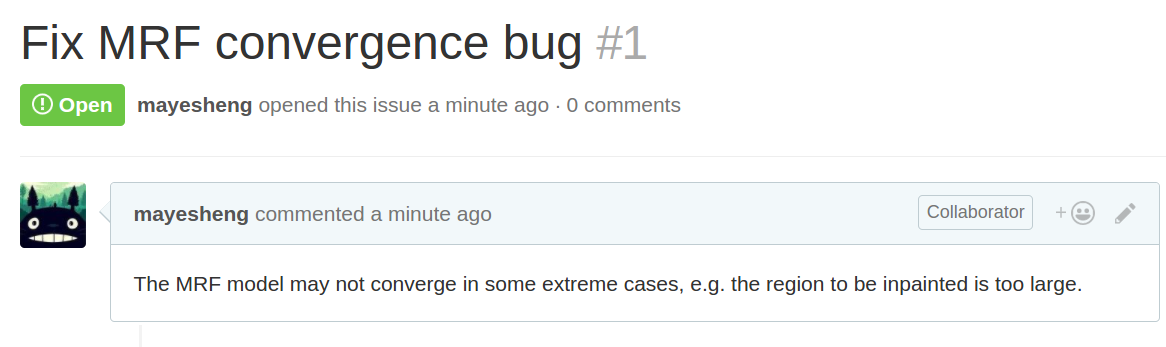
\includegraphics[width=10cm]{sc1.png}
    \caption{A sample issue tracker}
\end{figure}
Altogether we make about 50 commits and roughly 15000 lines of code.
